% !TEX root = ../my-thesis.tex
%
\chapter{Methods of acceleration}
\label{sec:acceleration}

Up until this chapter, most aspects of the algorithm we discussed build on papers that Wu et al. used as a basis during their research. Next, we introduce the main propositions they developed, which all contribute to making the algorithm faster and viable for real-time application. In order to accomplish this, the execution time of the algorithm has to be below $16.\overline{6}\text{ms}$ to be running at $60$ frames per second.

\section{Handling splash particles}
\label{sec:splashparticles}

\begin{figure}[h]
    \centering
    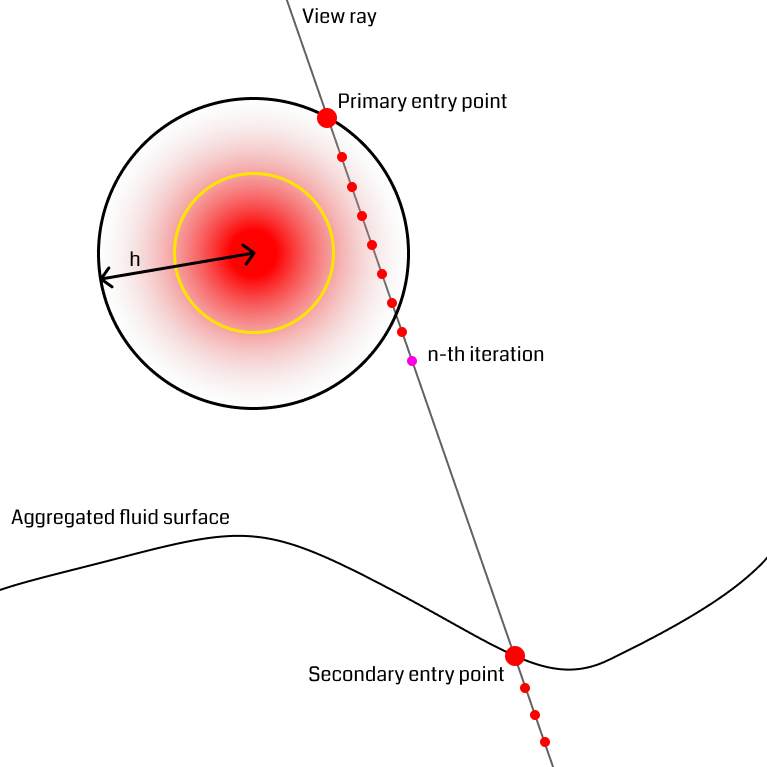
\includegraphics[width=0.75\textwidth]{my-gfx/figure-splash.png}
    \caption{The ray marching starts at the point extracted from the primary depth buffer. Here, the ray does not reach $\sigma$ (the iso-surface, indicated in yellow) in $n$ iterations. It can now skip to the point extracted from the secondary depth buffer which only aggregated particles were rendered to. The red gradient represents the kernel function of a particle.}
    \label{fig:splash}
\end{figure}

It is often the case that small bundles of particles fly up above the denser part of the fluid (Figure \myref{fig:splash}). Consider the rays starting at the outer rim of the splash particle's sphere. When traversing through the outer part of the sphere, they are unlikely to reach the density threshold $\sigma$ before exiting the sphere at the backside. In this situation, the ray would have to take a lot of steps to reach the next part of the fluid. The solution the authors suggest uses the previously mentioned secondary depth buffer $D_{agg}$ that only particles whose density exceeds a certain threshold are rendered to, omitting low-density areas like splash particles. When a ray reaches a certain number of steps and has not found an iso-surface yet, it computes a new position from the secondary depth buffer and continues from there, effectively skipping empty space and restarting near the fluid surface. This technique once more has the effect of reducing the number of ray marching steps.

\section{Adaptive step lengths}

The authors propose a data structure that helps reduce the number of steps during ray marching they call \textit{binary density grid} or \textit{density mask}. This enables the ray marcher to adapt the length of steps on the ray depending on the fluid's density in the surrounding area. To achieve this, a grid of cells is generated holding a boolean value indicating whether or not a surface can be expected in this cell.

Equation 1 of the paper states this criterion for every cell $c$:
\[
M_c := \begin{cases}
1 & \rho_c^{max} \geq \sigma, \\
0 & else
\end{cases}
\]
It is now the goal to determine an approximation of the maximum possible density $\rho_c^{max}$ inside the cell.

For every point $\textbf{r}_c$ inside cell $c$, we have (see equation 3 in \cite{Wu:2022})
\[
\rho(\textbf{r}_c) =
m \sum_{i \in N(\textbf{r}_c, h)} W(\textbf{r}_i - \textbf{r}_c) \leq
m N_c W(\textbf{0}) =: \rho_c^{max},
\]
where $N_c \geq |N(\textbf{r}_c, h)|$ is a constant approximation of the number of particles in and around the cell $c$. Note that $W$ has its global maximum at $\textbf{0} = (0, 0, 0)^T$.

The idea for determining $N_c$ is similar to the neighborhood search described in the chapter \textbf{Particle neighborhood and anisotropic kernels \myref{sec:particleneighborhood}}: If the cell size equals the particles' radius, only the $3 \times 3 \times 3$ neighborhood of each cell has to be taken into account. Wu et al. use a three-dimensional convolution on an array $N$ containing the number of particles per cell to approximate $N_c$. They give a two-dimensional example illustrating their idea. Let cell $c$ be at location $(x, y)$, then $N_{(dx,dy)}$ is the number of particles inside the cell located at $(x + dx, y + dy)$:
\[
N_c :=
\begin{bmatrix}
  N_{(-1,-1)} & N_{(0,-1)} & N_{(1,-1)} \\
  N_{(-1,0)} & N_{(0,0)} & N_{(1,0)} \\
  N_{(-1,1)} & N_{(0,1)} & N_{(1,1)} \\
\end{bmatrix}
* K
\]
with a "spatially separable" convolution kernel $K$ (see equation 5 in \cite{Wu:2022})
\[
K :=
\begin{bmatrix} b \\ a \\ b \end{bmatrix} \times
\begin{bmatrix} b & a & b \end{bmatrix} =
\begin{bmatrix}
b^2 & ab & b^2 \\
ab & a^2 & ab \\
b^2 & ab & b^2 \\
\end{bmatrix}
.
\]
For three dimensions, this expands to the three-dimensional tensor $K^{(3)}$ with two-dimensional slices $K^{(3)}_1, K^{(3)}_2, K^{(3)}_3$:
\[
K^{(3)}_1 = K^{(3)}_3 := b K =
\begin{bmatrix}
b^3 & ab^2 & b^3 \\
ab^2 & a^2b & ab^2 \\
b^3 & ab^2 & b^3 \\
\end{bmatrix},
\]
\[
K^{(3)}_2 := a K =
\begin{bmatrix}
ab^2 & a^2b & ab^2 \\
a^2b & a^3 & a^2b \\
ab^2 & a^2b & ab^2 \\
\end{bmatrix}.
\]
This convolution can once again run in parallel on the GPU, achieving computation times as low as $11\text{ms}$ for over $600,000$ particles (Table 2 in \cite{Wu:2022}).

$a, b < 1$ are parameters that have to be carefully chosen to be not too strict and not too loose for approximating $N_c$. The authors suggest to choose $a > b$ because the cells closer to the center are more important in the calculation and should have higher weights.

Once the grid is constructed, it is queried during ray marching before performing the expensive neighborhood search. In most cases, the query evaluates to false, meaning the position can be advanced to the intersection of the ray and the grid cell's axis-aligned bounding box. Through this technique, big parts of empty space can be skipped without the need to compute the density directly and notable performance benefits are achieved (we measured a speedup of around $1.2$, but this greatly depends on the scene and viewing angle).

Furthermore, the cells can be arranged in a tree-like structure and neighboring cells with the same value can be substituted for a larger one (Figure 3 of Wu et al. \cite{Wu:2022}). Again, this reduces the number of ray marching iterations by allowing to take bigger steps.


\section{Adaptive resolution}

Another method the authors propose is to reduce the number of rays cast into the scene adaptively. The question is how to minimize the loss of information that arises when shooting fewer rays. For flat fluid areas, information between samples can be generated using linear interpolation. So, when the flatness of a region exceeds a certain threshold, rays are only shot for every two pixels and the remaining ones are filled by interpolation.

As a measure of flatness, Wu et al. suggest using the variance of the values stored in the primary depth buffer $D$. The screen is divided into equally sized regions for which the variance is evaluated and the number of rays shot into this region is determined. Depending on two threshold values $\epsilon_1 < \epsilon_2$, either full resolution, half resolution or quarter resolution is used in that tile (see section 4.3 in Wu et al. \cite{Wu:2022}):
\begin{align*}
& \text{Var}(D) \in [0, \epsilon_1) \Rightarrow \text{quarter} \\
& \text{Var}(D) \in [\epsilon_1, \epsilon_2] \Rightarrow \text{half} \\
& \text{Var}(D) \in (\epsilon_2, \infty) \Rightarrow \text{full}
\end{align*}
Using adaptive resolution, the authors managed to achieve an approximate speedup of $1.5$ on a $1920 \times 1920$ screen with a dam break dataset with no drawbacks in image quality (Table 1 and Figure 7 of Wu et al. \cite{Wu:2022}).
